\documentclass[a4paper,11pt]{jsarticle}


% 数式
\usepackage{amsmath,amsfonts}
\usepackage{bm}
% 画像
\usepackage[dvipdfmx]{graphicx}


\begin{document}

\title{知能システム論 第3回レポート}
\author{阿部 桃大}
\date{\today}
\maketitle
\section{概要}
今回の課題ではポケモンの種族値のデータベースを用いて、PCAの後にk-meansを行い、3つのクラスタに分類する解析を行った。
また、ガウシアンカーネルを用いて同様にPCAの後にk-meansを行い、3つのクラスタに分類する解析を行った。

なお、解析元となるデータは、\texttt{https://www.kaggle.com/datasets/abcsds/pokemon}から取得した。

\section{実装}
本課題の実装は、\texttt{kadai.py}にて行った。このプログラムは、Pokemon.csvからポケモンの6つの種族値(H,A,B,C,D,S)を読み込み、上記の解析を行う。

コードの詳細については添付のコード内にコメントとして記載している。

\newpage

\section{解析結果}
以下に2つの手法を用いて行った解析の結果を示す。
% ここに結果を示す
% 2つの手法を並べて比較する

\begin{figure}[h]
  \begin{minipage}
    {0.5\hsize}
    \begin{center}
      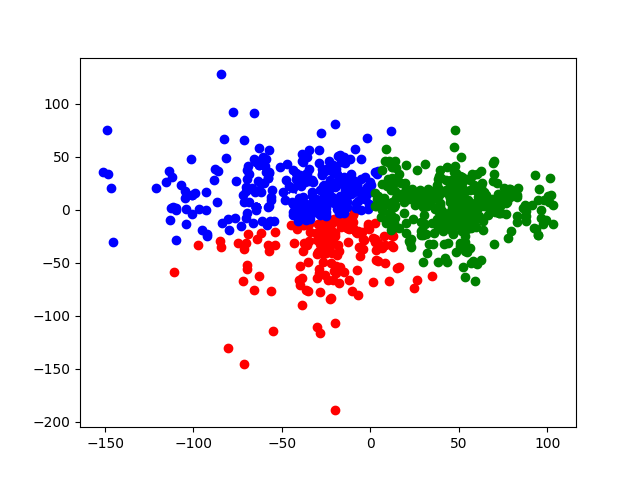
\includegraphics[width=7cm]{pca_and_kmeans.png}
    \end{center}
    \caption{PCAの後にk-meansを行った結果}
    \label{fig:PCA}
  \end{minipage}
  \begin{minipage}
    {0.5\hsize}
    \begin{center}
      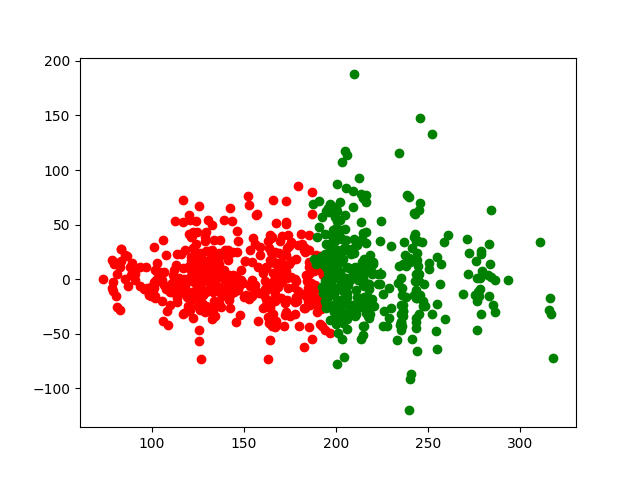
\includegraphics[width=7cm]{kernel_pca_and_kmeans.png}
    \end{center}
    \caption{ガウシアンカーネルを用いてPCAの後にk-meansを行った結果}
    \label{fig:PCA_gaussian}
  \end{minipage}
\end{figure}

\section{考察}
通常のPCA及びk-meansを用いた場合、図\ref{fig:PCA}のように、3つのクラスタに分類された。しかし、各クラスタの境界には多くのデータが含まれており、クラスタの分類がうまくいっていないと考えられる。

一方で、ガウシアンカーネルを用いたPCA及びk-meansを用いた場合、図\ref{fig:PCA_gaussian}のように、2つのクラスタに分類された。この結果においても、各クラスタの境界には多くのデータが含まれており、クラスタの分類がうまくいっていないと考えられる。
ここで、本来は3つのクラスタに分類されるはずのデータが2つのクラスタに分類されたことから、ガウシアンフィルタを用いるとこのデータが本質的に2つのクラスタに分類されるような特性を持つものだと考えられる。

最後に各クラスタの意味についても軽く考察しておく。

通常のPCA及びk-meansを用いた場合、クラスタ1はHPが高く、クラスタ2はHPが低いという特徴が見られる。また、ガウシアンカーネルを用いたPCA及びk-meansを用いた場合、x軸は(-0.30,-0.49,-0.38,-0.51,-0.39,-0.32)の固有ベクトルに対応し、y軸は(-0.04,-0.07,-0.70,0.38,-0.17,0.58)の固有ベクトルに対応する。したがってxが高いポケモンは全体的に種族値が低い傾向にあり、未進化ポケモンなどが多く該当すると思われる。yが高いポケモンは特攻が低く、防御と素早さが高い傾向にある。つまり、緑色は未進化ポケモンなどの低種族値ポケモンで、青色は特攻が低く、防御と素早さが高いポケモン、逆に赤色は特攻が高く、防御と素早さが低いポケモンと考えられる。

ガウシアンカーネルを用いた手法のほうでは二つのクラスタを分けているのはx成分であるが、これも上の場合と同様に(0.43,0.38,0.38,0.41,0.45,0.38)の固有ベクトルに対応し、全体的な種族値を表すパラメータであるといえる。すなわち、赤色は全体的に種族値が低い未進化などのポケモン、緑色は全体的に種族値が高い伝説ポケモンや最終進化ポケモンなどと考えられる。
\end{document}
